\documentclass[11pt]{article}
\usepackage[letterpaper,margin=1in]{geometry}
\usepackage{times}
\usepackage[T1]{fontenc}
\usepackage{microtype}
\usepackage[round,numbers]{natbib}
\usepackage{booktabs}
\usepackage{graphicx}
\usepackage{amsmath,amssymb}
\usepackage{xcolor}
\usepackage[hidelinks]{hyperref}
\usepackage{caption}
\usepackage{subcaption}
\usepackage{enumitem}
\usepackage{fancyvrb}
% Let long \texttt{} file paths break across lines; without this, a paragraph that
% names three paths runs into the margin and cannot be fixed by stretching spaces.
\usepackage[htt]{hyphenat}
\usepackage{titlesec}
\captionsetup{font=small,labelfont=bf}
% Long \texttt{} paths are unbreakable; let TeX stretch spaces instead of running
% into the margin on the few paragraphs that quote several of them at once.
\setlength{\emergencystretch}{2em}
\setlist[itemize]{leftmargin=1.2em,itemsep=1pt,topsep=3pt}
\titleformat{\section}{\large\bfseries}{\thesection}{0.6em}{}
\titleformat{\subsection}{\normalsize\bfseries}{\thesubsection}{0.5em}{}
\newcommand{\arb}{\textsc{Agent Recovery Bench}}
\newcommand{\ttd}{\texttt{TTD}}
\newcommand{\ttr}{\texttt{TTR}}
% Auto-generated by paper/analysis.py -- do not edit.
\newcommand{\NumPairs}{1,125}
\newcommand{\NumHarmful}{861}
\newcommand{\NumEpisodes}{4,920}
\newcommand{\InertPct}{23.5}
\newcommand{\RecNoRecovery}{0.0}
\newcommand{\RecRetry}{0.0}
\newcommand{\RecRules}{60.9}
\newcommand{\RecModel}{51.3}
\newcommand{\AucRules}{0.772}
\newcommand{\AucSupervised}{0.762}
\newcommand{\AucRulesBlackbox}{0.787}
\newcommand{\ClaimedPct}{45.6}
\newcommand{\VerifiedPct}{28.0}
\newcommand{\FalseClaimPct}{38.4}
\newcommand{\FalseClaimN}{603}
\newcommand{\NaturalDetected}{64.1}
\newcommand{\NaturalRecovery}{89.7}
\newcommand{\NaturalAgreement}{92.0}
\newcommand{\NaturalN}{39}
\newcommand{\CommRecovery}{82.2}
\newcommand{\SingleRecovery}{31.9}
\newcommand{\MultiRecovery}{20.3}
\newcommand{\DiffRetryonlyVsNorecovery}{+0.0}
\newcommand{\DiffRetryonlyVsNorecoveryLo}{+0.0}
\newcommand{\DiffRetryonlyVsNorecoveryHi}{+0.0}
\newcommand{\DiffRulebasedVsRetryonly}{+60.9}
\newcommand{\DiffRulebasedVsRetryonlyLo}{+57.9}
\newcommand{\DiffRulebasedVsRetryonlyHi}{+65.3}
\newcommand{\DiffRulebasedVsNorecovery}{+60.9}
\newcommand{\DiffRulebasedVsNorecoveryLo}{+57.9}
\newcommand{\DiffRulebasedVsNorecoveryHi}{+65.3}
\newcommand{\DiffModelbasedVsRulebased}{-9.5}
\newcommand{\DiffModelbasedVsRulebasedLo}{-13.6}
\newcommand{\DiffModelbasedVsRulebasedHi}{-6.2}
\newcommand{\RulesPrecision}{66.9}
\newcommand{\RulesRecall}{41.9}
\newcommand{\RulesFone}{51.5}
\newcommand{\RulesTypeAcc}{34.6}
\newcommand{\SupPrecision}{48.8}
\newcommand{\SupRecall}{86.2}
\newcommand{\SupFone}{62.3}
\newcommand{\SupTypeAcc}{51.6}
\newcommand{\SupThreshold}{0.75}
\newcommand{\DetTrainRows}{5,583}

\newcommand{\BlackboxRecRules}{34.6}
\newcommand{\BlackboxRecRulesLo}{30.0}
\newcommand{\BlackboxRecRulesHi}{39.5}
\newcommand{\BlackboxDetRules}{88.5}
\newcommand{\BlackboxRecModel}{28.2}
\newcommand{\EarlyN}{501}
\newcommand{\EarlyRec}{71.7}
\newcommand{\EarlyGap}{20.9}
\newcommand{\LateN}{325}
\newcommand{\LateRec}{50.8}
\newcommand{\EarlyAlarmRate}{0.0}

% Auto-generated by paper/analysis.py -- do not edit.
\newcommand{\LLMMcNemarB}{80}
\newcommand{\LLMMcNemarC}{0}
\newcommand{\LLMMcNemarPairs}{240}
\newcommand{\LLMMcNemarP}{\ensuremath{1.7\times10^{-24}}}
\newcommand{\LLMAvailable}{1}
\newcommand{\LLMModel}{qwen2.5-coder:7b}
\newcommand{\LLMPairs}{240}
\newcommand{\LLMRecovery}{27.5}
\newcommand{\LLMRecoveryLo}{23.8}
\newcommand{\LLMRecoveryHi}{63.3}
\newcommand{\LLMRuleRecovery}{60.8}
\newcommand{\LLMRuleRecoveryLo}{58.9}
\newcommand{\LLMRuleRecoveryHi}{80.0}
\newcommand{\LLMPairedDelta}{+33.3}
\newcommand{\LLMPairedLo}{+16.7}
\newcommand{\LLMPairedHi}{+35.0}
\newcommand{\LLMCalls}{42}
\newcommand{\LLMDecisions}{225}
\newcommand{\LLMMisuse}{95.5}
\newcommand{\LLMRuleMisuse}{95.5}
\newcommand{\LLMStale}{80.0}
\newcommand{\LLMRuleStale}{80.0}
\newcommand{\LLMRuleContainment}{100.0}
\newcommand{\LLMRetryPct}{60.4}
\newcommand{\LLMFollowPct}{0.0}
\newcommand{\LLMFallbacks}{0}
\newcommand{\LLMContainment}{25.0}

% Auto-generated by paper/analysis.py -- do not edit.
\newcommand{\StatsPairs}{861}
\newcommand{\RuleVsModelB}{104}
\newcommand{\RuleVsModelC}{22}
\newcommand{\RuleVsModelP}{\ensuremath{<}0.001}
\newcommand{\RuleVsModelPHolm}{\ensuremath{<}0.001}
\newcommand{\RuleVsNoRecoveryP}{\ensuremath{<}0.001}
\newcommand{\RuleVsNoRecoveryPHolm}{\ensuremath{<}0.001}
\newcommand{\ModelVsNoRecoveryP}{\ensuremath{<}0.001}
\newcommand{\HolmPolicyTests}{6}
\newcommand{\HolmClassTests}{7}
\newcommand{\HolmClassSignificant}{2}
\newcommand{\HolmFamilyTests}{4}
\newcommand{\HolmFamilySignificant}{3}

% Auto-generated by paper/analysis.py -- do not edit.
\newcommand{\AucRulesLo}{0.749}
\newcommand{\AucRulesHi}{0.789}
\newcommand{\RulesFoneLo}{50.0}
\newcommand{\RulesFoneHi}{53.4}
\newcommand{\RulesPrecisionLo}{66.2}
\newcommand{\RulesPrecisionHi}{68.1}
\newcommand{\RulesRecallLo}{40.1}
\newcommand{\RulesRecallHi}{44.8}
\newcommand{\DetectionClusters}{3}


\title{\textbf{Agent Recovery Bench: Measuring Whether Failures Are Detected\\
Early and Repaired Reliably in Tool-Using and Multi-Agent Workflows}}
\author{Anonymous submission}
\date{}

\begin{document}
\maketitle

\begin{abstract}
Task-success leaderboards tell us whether an agent finished, not why it failed, whether it
noticed, or whether the repair was worth its cost. We introduce \arb{}, a benchmark for the
\emph{detection and recovery} half of agent reliability. \arb{} contributes (i) a compact
seven-class failure taxonomy---misuse/invalid arguments, stale state, contradictory evidence,
planning error, communication failure, objective drift, and unrecoverable external error---whose
classes are defined by the \emph{signal} that identifies them and the \emph{operator} that repairs
them; (ii) four deterministic tool environments (refunds, data migration, inventory accounting, and
a three-role procurement desk) in which success is verified from world state rather than from the
agent's report; (iii) a controlled fault-injection harness that replays an identical reference
trajectory with and without a scheduled fault, screening out non-harmful injections so that
detection and recovery are measured only where failure actually changes the outcome; and (iv) a
protocol comparing no recovery, retry-only, rule-based, and model-based recovery under a fixed price
sheet. Across \NumHarmful{} harmful task--fault pairs and \NumEpisodes{} evaluated episodes, a
rule-based detector reaches step-level AUC \AucRules{} (F1 \RulesFone{}), and the rule-based
recovery policy repairs \RecRules\% of harmful failures against \RecNoRecovery\% with no recovery
and \RecRetry\% with retries alone; a learned ranker reaches \RecModel\% and does not beat the
canonical mapping. Recovery is strongly class-dependent (from \emph{misuse} and
\emph{contradictory evidence} at roughly 96\% down to \emph{planning error} at 41\% and
\emph{objective drift} at 52\%) and timing-dependent: failures detected before they propagate are
recovered \EarlyRec\% of the time versus \LateRec\% when detection is late. Agents claim success
\ClaimedPct\% of the time and succeed \VerifiedPct\% of the time, so
\FalseClaimPct\% of success claims are wrong---a gap that any evaluation based on self-report would
score as progress. All environments are simulated: \arb{} measures \emph{relative} reliability
under controlled faults, not production reliability.
\end{abstract}

\section{Introduction}

Agents built on language models now plan, call tools, and delegate to other agents. The dominant
way we measure them is task success: did the ticket get refunded, did the migration finish, did the
buy order go through \citep{yao2024taubench,liu2023agentbench,zhou2023webarena}. Success rates are
useful but they collapse three very different competencies into one bit. An agent that never
encounters a fault, an agent that encounters a fault and silently routes around it, and an agent
that hits a fault, notices, and repairs it are all scored as ``1''. An agent that fails because a
tool returned a stale read and an agent that fails because it misread the objective are both
scored as ``0''.

The consequence is that we cannot answer the question practitioners actually ask when an agent
breaks in production: \emph{would it have noticed?} A reliability claim about an agent is a claim
about a closed loop---detect, diagnose, repair, verify---and current benchmarks only score the last
step's shadow, whether the final answer happened to be right. Worse, the loop can look closed when
it is not: our agents assert success in their own trajectory \emph{far} more often than they
achieve it (Sec.~\ref{sec:results}), so a judge that reads the transcript will over-credit them.

This paper asks a narrow, measurable question:

\begin{quote}\itshape
Can agent failures be detected early and recovered from reliably, and which failure signals predict
successful recovery in multi-step tool-using and multi-agent workflows?
\end{quote}

\noindent We answer it with \arb{}, a benchmark that extends failure \emph{counting} into failure
\emph{handling} under control. Our contributions:

\begin{enumerate}[leftmargin=1.4em]
\item \textbf{A signal-defined taxonomy} of seven classes---misuse (invalid arguments), stale state,
contradictory evidence, planning error, communication failure, objective drift, and unrecoverable
external error---each with a characteristic observation signature, a canonical remediation operator,
and an explicit recoverability status (Table~\ref{tab:taxonomy}). The taxonomy is defined by what
you can \emph{see} and what you would \emph{do}, not by which module we believe is at fault, which
keeps labels independent of any particular agent architecture.

\item \textbf{Four deterministic tool environments} with verifiable world state (refund desk,
dual-store migration, inventory accounting with an auditable invariant, three-role procurement with
a message bus). Outcomes are read from state, never from the agent's prose. Faults are injected on a
schedule aligned to the step that calls the targeted tool, and every trajectory stores expected
state, observed state, the mismatch, and the resulting harm.

\item \textbf{An inert-fault screen.} We run every (task, fault) pair with no recovery first.
\InertPct\% of injections leave the task outcome unchanged. These are excluded from detection and
recovery denominators, so a model is never rewarded for ``detecting'' a fault that did not matter
and recall is not inflated by faults no monitor could be blamed for missing.

\item \textbf{A four-way recovery comparison}---no recovery, retry-only, rule-based (canonical
operators), and model-based (learned operator selection)---scored on the same episodes with
auto-verified outcomes, cluster-bootstrap confidence intervals over task templates, and a fixed
price sheet so that cost is part of the result.

\item \textbf{Release} of the dataset, deterministic harness, baseline detector and evaluator,
optional recovery ranker, reference agents, fixed configs, and a leaderboard protocol with pinned
versions (Sec.~\ref{sec:release}).
\end{enumerate}

\paragraph{What we find.} (i) Detection is easier than repair. A 13-rule monitor over
heterogeneous signals reaches AUC \AucRules{}, but even with oracle-quality detection the rule-based
policy repairs only \RecRules\% of harmful failures. (ii) Repair is class-dependent in a way that
inverts intuition: mechanically ``hard'' classes such as contradictory evidence are repaired at
96\%, while \emph{planning error} (41\%) and \emph{objective drift} (52\%)---the classes that
require knowing what the task was supposed to be---are where recovery collapses. (iii) Timing
carries real signal: episodes detected before the fault propagates are recovered \EarlyRec\% of the
time, versus \LateRec\% for late detection. (iv) A learned operator ranker trained off-policy on
logged decisions reaches \RecModel\%, i.e.\ it does not beat the hand-written canonical mapping; we
report this negative result rather than tuning it away. (v) Multi-agent episodes recover less often
than single-agent episodes on the same fault set (\MultiRecovery\% vs \SingleRecovery\%), and
coordination faults are recoverable only when the message bus is re-synchronised---a repair
operator that has no single-agent analogue.

\paragraph{What this is not.} \arb{} is entirely simulated. It does not measure production
reliability, and relative ordering under injected faults need not transfer to the messy failures of
real deployments. The reference agents are scripted workflow executors with a known standard
operating procedure and no oracle access; one experiment replaces the recovery \emph{controller}
with a local 7B language model (Sec.~\ref{sec:results}), but no frontier model plans the tasks, and
no frontier model is evaluated here. We state what this buys (exact control, exact verification,
exact replay) and what it costs (external validity) in Sec.~\ref{sec:limits}.

\section{Related Work}

\paragraph{Task-success agent benchmarks.} $\tau$-bench \citep{yao2024taubench} established the
modern shape of tool-agent evaluation: a domain database, a user simulator, and programmatic
comparison of the final database state against a goal state, with the $\text{pass}^k$ metric
measuring consistency across repeated trials. $\tau^2$-bench \citep{taubench2} extends this to
dual-control settings where the user also acts on the shared world. WebArena
\citep{zhou2023webarena}, Mind2Web \citep{deng2023mind2web}, AgentBench \citep{liu2023agentbench},
GAIA \citep{mialon2023gaia}, ToolLLM \citep{qin2023toolllm} and Gorilla \citep{patil2023gorilla}
similarly score end states. Our verifier inherits $\tau$-bench's insistence on state comparison,
but the unit of analysis is not a task---it is a \emph{fault} inside a task, with a matched
fault-free twin.

\paragraph{Failure taxonomies and attribution.} Recent work has begun to catalogue how agents fail.
Zhang et al.~\citep{zhang2025whowhen} build a step-level dataset of annotated failure points and study
\emph{who} is responsible in multi-agent systems; Cemri et al.~\citep{cemri2025mast} derive a multi-agent failure
taxonomy from traces and report that verification and inter-agent misalignment dominate.
Suzgun et al.~\citep{suzgun2025failuretaxonomy} taxonomise ``thinking failures'' in reasoning models;
Zhu et al.~\citep{zhu2025where} propose a trajectory-level taxonomy. \arb{} differs in what the taxonomy is
\emph{for}. Those taxonomies describe causes; ours is built to be \emph{actionable}---each class
carries the operator that repairs it and the signal that reveals it---and every class is paired with
a controlled injection program so that a label is a reproducible intervention, not an annotator's
judgement. This makes detection and recovery separately scorable, and it makes disagreement
measurable (a detector that labels a stale read as a planning error is penalised as such).

\paragraph{Self-correction and reflection.} Reflexion \citep{shinn2023reflexion}, self-debugging
\citep{chen2024selfdebug} and self-repair \citep{olausson2024selfrepair} report gains from
model-generated critique. A parallel literature is sceptical: Huang et al.~\citep{huang2024selfcorrect} and Kamoi et al.~\citep{kamoi2024selfcorrection} show that models often cannot correct reasoning without external
signal, and that apparent gains come from the harness. \arb{} speaks directly to this: our
retry-only baseline, which is the degenerate self-correction loop, recovers \RecRetry\%. Repair
requires a \emph{diagnosis}, and the diagnosis requires evidence the model did not generate.

\paragraph{Process supervision and step-level verification.} Process reward models
\citep{lightman2023prm,uesato2022safety,cobbe2021gsm8k} score intermediate steps for correctness.
Our detector is a step-level monitor in that tradition but with a different label semantics: the
target is not ``is this step correct'' but ``is the trajectory in a faulty state, and of which
class'', which is a state-estimation problem rather than a preference-learning one.

\paragraph{Fault injection and chaos engineering.} Injecting faults to measure resilience is
long-standing practice in dependable systems \citep{hsueh1997fault,scully2015fault} and in chaos
engineering \citep{basiri2016chaos,lightstone2004chaos}. \arb{} is, structurally, a fault-injection
campaign for agent trajectories: deterministic schedules, matched controls, and harm screening. The
difference is that the ``system under test'' is a stochastic policy over tool calls and the
observable is a natural-language-adjacent trajectory, so the fault must be expressed as a
perturbation of \emph{observations} and \emph{tool effects} rather than of memory bits.

\paragraph{Benchmark critique.} Raji et al.~\citep{raji2021ai} argue benchmarks are boundary objects whose
construct validity must be argued, not assumed. We take that seriously: Sec.~\ref{sec:limits} is
explicit about which claims the design supports (relative ranking under controlled faults) and which
it does not (absolute production reliability). Amodei et al.~\citep{amodei2016concrete} and Hendrycks et al.~\citep{hendrycks2021ethics} list safe exploration and oversight as core problems; a monitor that
detects and contains rather than repairs is a small concrete instance of both.

\section{The \arb{} Benchmark}\label{sec:bench}

\subsection{A compact, signal-defined failure taxonomy}

\arb{} uses exactly seven failure classes. The design constraint was that a class must be
(1) \emph{observable}---there exists a monitor-visible signal that discriminates it; (2)
\emph{injectable}---we can realise it deterministically inside a tool environment; and (3)
\emph{actionable}---a specific repair operator is prescribed. Table~\ref{tab:taxonomy} lists them
with detectability, canonical remediation, and recoverability.

\begin{table*}[t]
\centering
\small
\caption{The \arb{} failure taxonomy. \emph{Detectability} is a property of the signal, not of a
model: \emph{surface} classes are visible in error codes or version counters, \emph{latent} classes
require cross-referencing evidence or the objective specification. \emph{Canonical remediation} is
the operator a domain expert prescribes; it defines the rule-based reference policy.}
\label{tab:taxonomy}
\begin{tabular}{@{}lllll@{}}
\toprule
Class & Detectability & Track & Canonical remediation & Recoverable \\
\midrule
invalid\_arguments & surface & single+multi & \texttt{revalidate\_args} & yes \\
stale\_state & surface & single+multi & \texttt{re\_read\_authoritative} & yes \\
contradictory\_evidence & latent & single+multi & \texttt{refresh\_state} & yes \\
planning\_error & latent & single+multi & \texttt{replan} & yes \\
communication\_failure & surface & multi & \texttt{resync\_message} & yes \\
objective\_drift & latent & single+multi & \texttt{reanchor\_objective} & yes \\
unrecoverable\_external\_error & surface & single+multi & \texttt{escalate\_abort} & no (contain) \\
\bottomrule
\end{tabular}
\end{table*}

The split between \emph{surface} and \emph{latent} is the load-bearing distinction. A surface class
announces itself: the tool returns a schema violation, or a read carries a version counter older
than the current one. A latent class does not: contradictory evidence is two {\em individually
plausible\/} values for the same field, planning error is a well-formed step that serves the wrong
subgoal, and objective drift is a locally sensible action that no longer serves the stated goal.
Latent classes require an internal model of what the task \emph{should} be doing, which is precisely
what a monitor built only on error codes lacks.

\texttt{escalate\_abort} is deliberately not a repair. For an unrecoverable external error the
correct behaviour is to stop mutating, leave the world consistent, and hand off. We therefore score
containment (no successful mutation after the fault) separately from recovery, and we never count a
containment as a recovery.

\subsection{Environments and the reference agent}

Four families, each a deterministic Python world with a version counter and a bounded history:

\begin{itemize}
\item \textbf{Refund desk (\texttt{tickets}).} Support tickets with a refund policy whose arithmetic
(constituent caps, prior refunds, order totals) must be recomputed each time. The SOP includes a
check-then-act re-read before moving money, which makes stale-read faults physically costly.
\item \textbf{Dual-store migration (\texttt{migration}).} A source store and a migrated store; the
agent copies records and must reconcile. Background writers touch only objects the agent has not
read, so silent lost updates are possible and a completion claim can be wrong.
\item \textbf{Inventory accounting (\texttt{inventory}).} An auditable invariant
(\texttt{on\_hand} $+$ $\sum$ \texttt{adjustments} $=$ \texttt{ledger}) plus a \texttt{close\_period}
gate. Corrections are made by posting compensating adjustments, never by editing history.
\item \textbf{Procurement desk (\texttt{procurement}).} Three roles---planner, buyer, verifier---on a
message bus with an incremental order protocol (cancel and re-issue is the repair path). This is the
multi-agent family; the others are single-agent.
\end{itemize}

The \emph{reference agent} is a scripted workflow executor. It knows the procedure and the
environment's affordances (\texttt{solve}/\texttt{next\_step}) but has \emph{no access to ground
truth}: every tool argument is derived from that role's belief, i.e.\ from observations it has
actually received and applied. This design choice is what makes the hard classes real. If the
argument were computed from the world, a stale read would be harmless; because it is computed from
belief, a stale read propagates into the next mutation. Similarly, a dropped message is not merely
``an event we log''---the receiving role's belief never updates, so it acts on the wrong sender or
the wrong quantity.

Agent-side ``natural'' faults (omitting a required verification step, using a superseded value,
mis-ordering a two-phase mutation) can be switched on to produce failures that were not injected by
the harness; we use them as a provenance-shift check (Table~\ref{tab:natural}).

\subsection{Tasks, splits, and leakage control}

A task is a (family, template, configuration, seed) tuple. Templates define the procedure shape;
configurations vary concurrency, dataset size, and which optional branches fire. Splits hold out
both:

\begin{itemize}
\item \textbf{train} --- templates A/B $\times$ configs 1--3;
\item \textbf{dev} --- templates A/B $\times$ config 5;
\item \textbf{test-id} --- templates A/B $\times$ config 6 (unseen configuration, higher concurrency);
\item \textbf{test-ood} --- template C (unseen template).
\end{itemize}

Detector thresholds are tuned on \emph{dev}; the supervised detector and the recovery ranker are fit
on \emph{train} only. Nothing in test-id or test-ood is seen during fitting, and fault schedules are
generated per task from a seeded RNG so that memorising a schedule is not a viable strategy.

\subsection{Fault injection as a program}

Each class is realised by a small \emph{operator program} applied at a scheduled step: a sequence of
primitive perturbations (corrupt an argument, re-serve an older snapshot, plant a conflicting value,
suppress a message, drop a subgoal, swap the objective, raise a terminal tool error). \texttt{inject\_at}
is aligned to the step that calls the targeted tool---the last read of that field, or the first
mutation---so a scheduled fault is always actually exercised. The same program is used for every
family, which is what lets us pool classes across environments.

\subsection{Harm screening}

Not every injection changes the outcome. A stale read that is never used, or a duplicated message
that is idempotent, leaves the task successful. We therefore run every (task, fault) pair under
\texttt{no\_recovery} and keep only pairs where the task actually fails: \NumHarmful{} of
\NumPairs{} (\InertPct\% inert, discarded). This has two effects. It defines the denominator, so
``recovery rate'' means ``fraction of \emph{harmful} faults repaired''. And it is conservative for
detection: faults that are present but harmless are never counted as false negatives or as
detections. The cost is a selection effect---the retained set is biased toward faults with large
downstream reach---which we discuss in Sec.~\ref{sec:limits}.

\section{Harnes, Monitors, and Policies}\label{sec:method}

\subsection{Episode loop and label semantics}

An episode is a (task, fault, monitor, policy) tuple. The harness steps the reference agent; at each
step the environment returns an observation, the monitor scores it, and any alarm is handed to the
policy, which may enqueue a \emph{recovery program}---a short sequence of operator steps executed
before the agent's own next step. Recovery therefore costs real steps and real tool calls; it is
never a free relabelling of the transcript.

Every step carries: the tool call, its arguments, expected state, observed state, whether they
matched, a vector of monitor features, token counts, latency, and a USD cost under a versioned price
sheet (\texttt{arb-price-2026.11}) with deterministic jitter. A trajectory additionally carries the
fault plan (class, injection step), the detection point, the recovery action taken, the number of
retries, and the verified outcome.

Two label conventions matter and are easy to get wrong:

\begin{itemize}
\item \textbf{Detection is only counted from the injection step onward.} An alarm that fires before
the fault exists is a false alarm, not a lucky early detection. In practice this turned the
``time-to-detection'' distribution from contaminated to clean (Fig.~\ref{fig:ttd}), and the residual
early-alarm rate on the harmful set is \EarlyAlarmRate\%.
\item \textbf{Success is read from world state.} The agent's own claim is recorded as a separate
field and is never consulted by the grader. This is what makes the self-report gap in
Sec.~\ref{sec:results} measurable.
\end{itemize}

\subsection{Monitor features}

Nineteen features are computed per step, grouped into families: error codes and argument-schema
violations; version staleness (observed version lag, stale flag); cross-source disagreement
(conflict flag, disagreement count); communication (message lost, sender mismatch, unacknowledged);
policy conformance (mutation without a prior read of the mutated field, re-read violations);
progress (no-progress runs, repeated identical calls, retry streak); and cost pressure
(tokens and latency relative to the task's expectation). Features are computed from the observable
trace only: no feature reads the fault plan, the injection step, the grader verdict, or expected
state.

The supervisor is evaluated under two regimes. \emph{Instrumented} exposes the harness telemetry
flags (staleness, conflict, message-loss). \emph{Blackbox} zeroes them, leaving only error strings,
payloads, version counters and timing---i.e.\ what an external observer with no cooperation from
the runtime would see. The gap between regimes is the \emph{detectability gap}, and it is the honest
measure of how much a deployment can expect from a monitor that cannot instrument its own tools.

\subsection{Detectors}

\paragraph{Rule detector.} Thirteen rules over the feature families, each mapping a conjunction of
signals to a class with a confidence; the step score is the maximum over rules. Rules are
hand-written from the taxonomy, not tuned on the test splits.

\paragraph{Supervised detector.} A multinomial logistic regression over the 19 features (8 classes
including \emph{none}), trained in numpy with class balancing and L2. It is deliberately small: with
a few thousand labelled steps we are interested in whether the feature set carries signal, not in
winning a modelling contest. The decision threshold is swept on \emph{dev} to maximise F1
(selected $\tau=\SupThreshold$), and calibration is reported as ECE and Brier score since a monitor
that is badly calibrated will flood the policy with false alarms.

\subsection{Recovery policies}

\begin{itemize}
\item \textbf{No recovery.} Detector present, alarms ignored. This is the ``aggressive agent''
baseline and defines harm.
\item \textbf{Retry only.} On tool error, re-issue the same call up to a budget. This is the
degenerate self-correction loop, and it is the baseline that Reflexion-style methods must beat.
\item \textbf{Rule-based.} Detected class $\rightarrow$ canonical operator program
(Table~\ref{tab:taxonomy}), with guards: no more than one recovery per detected event, a repeated
-failure guard that escalates after a second identical failure, and no retries after the budget.
\item \textbf{Model-based.} A learned \emph{recovery action ranker} chooses between the canonical
repair for the detected class and a clean containment. The ranker is a set of per-operator logistic
value models, $P(\text{success}\mid a, x)=\sigma(w_a^\top x + b_a)$, over the posterior class
distribution, the alarm score, step pressure, error/staleness/conflict flags, retry streak and
retries used. Per-operator heads are necessary: a single model over action one-hots has no
action$\times$feature interaction, so its argmax is constant across all inputs and it degenerates to
``which action is best on average''. Operators with fewer than 25 logged executions are not
rankable and are excluded from the candidate set rather than being scored from a prior.
\end{itemize}

The ranker is fit on \emph{deliberate} decisions only---logged recovery choices from the rule-based
policy on the train split. Blind retries are excluded because they are not a choice of operator, and
including them teaches the model ``retry is bad'' as a global prior. This is off-policy learning
from a single logging policy, and it is the main reason we expect the learned policy to underperform
(Sec.~\ref{sec:results}); we report it as a boundary result rather than tuning it into a win.

\subsection{Metrics, intervals, and cost}

\paragraph{Detection.} Step-level labels (is a fault active at this step) give precision, recall, F1
and threshold-free AUC; class accuracy among positive steps measures whether the monitor knows
\emph{which} failure it is. Event-level recall asks whether the fault was ever detected at all.

\paragraph{Recovery.} Recovery rate conditional on class, plus attempt rate (did the policy try),
containment rate (for unrecoverable faults: no successful mutation after the fault), and
time-to-detection (\ttd) and time-to-recovery (\ttr) in steps.

\paragraph{Propagation.} Corrupted-step count (steps whose observed state diverges from expected)
and downstream-impact count (steps that were still wrong after the fault window), reported per
policy and per class.

\paragraph{Cost.}\label{sec:cost} Tool calls, tokens, wall-clock latency and USD per episode, plus USD per
\emph{recovered} episode---the amortised price of a repair, which is the number a deployment
actually budgets.

\paragraph{Intervals.} All intervals are 95\% cluster bootstrap \citep{efron1993bootstrap} resampling
\emph{task templates}, not episodes: episodes sharing a template share the procedure and the fault
schedule shape, so treating them as independent would understate uncertainty. Policy comparisons use
a paired bootstrap over templates on the same episode set. Single-episode proportions use Wilson
intervals \citep{wilson1927}.

\section{Results}\label{sec:results}

All numbers below come from \texttt{results/report\_main.json}, produced by
\texttt{scripts/run\_experiments.py} at the pinned commit, and are inserted into this document by
\texttt{paper/analysis.py}. The evaluated grid is \NumPairs{} task--fault pairs
(\NumHarmful{} harmful) over \NumEpisodes{} episodes.

\subsection{Detection is easier than repair}

\begin{table}[t]
\centering\small
\caption{Failure detection at the step level. Precision, recall and F1 are
computed on \emph{step-level} labels (is a fault active at this step?), so a
detector that fires every step scores high recall and low precision. AUC is
threshold-free. \emph{Type} is the accuracy of the predicted class among
positive steps. \emph{Instrumented} exposes harness telemetry flags;
\emph{blackbox} hides them, leaving only error codes, payloads, version
counters and timing.}
\label{tab:detection}
\begin{tabular}{@{}llcccccc@{}}
\toprule
Detector & Monitor & Prec. & Rec. & F1 & AUC & Type & Steps \\
\midrule
Rules & instrumented & 66.9 & 41.9 & 51.5 & 0.772 & 34.6 & 24,175 \\
Rules & blackbox & 86.7 & 32.0 & 46.7 & 0.787 & 22.1 & 1,094 \\
Supervised & instrumented & 48.8 & 86.2 & 62.3 & 0.762 & 51.6 & 11,193 \\
Supervised & blackbox & 46.0 & 81.0 & 58.7 & 0.750 & 39.9 & 1,060 \\
\bottomrule
\end{tabular}
\end{table}


The rule detector reaches AUC \AucRules{} (F1 \RulesFone\%, precision \RulesPrecision\%,
recall \RulesRecall\%), and the supervised detector is comparable (AUC \AucSupervised{}, F1
\SupFone\%, type accuracy \SupTypeAcc\% vs \RulesTypeAcc\% for rules). With cluster-bootstrap
intervals the rule monitor's step-level F1 is \RulesFone\% [\RulesFoneLo, \RulesFoneHi] and AUC
\AucRules{} [\AucRulesLo, \AucRulesHi] over \DetectionClusters{} templates
(Table~\ref{tab:detection_ci}); the intervals are wide because whole templates are resampled,
which is the honest resolution of a grid with three of them. Two things are worth
separating. First, aggregate AUC is respectable but \emph{class} accuracy is only around
35--50\%, i.e.\ the monitor usually knows that something is wrong and often does not know what.
Since the recovery policy is indexed by class, that confusion is expensive downstream: a stale read
labelled as a planning error triggers a replan that does not re-read, and the failure survives the
repair. Second, hiding the telemetry flags (blackbox) barely dents AUC (\AucRulesBlackbox{} for
rules, versus \AucRules{} instrumented; Fig.~\ref{fig:gap}) but does cost detection \emph{coverage}
in the recovery loop, because the latent classes lose their most reliable evidence. That cost is
large: with the identical rule detector and rule-based policy, a black-box monitor recovers
\BlackboxRecRules\% [\BlackboxRecRulesLo{}, \BlackboxRecRulesHi{}] of harmful faults, against
\RecRules\% when the runtime exposes its own staleness, conflict and message-loss telemetry. In
other words the ordering of a leaderboard entry is stable across regimes, but the absolute
reliability a deployment can expect is not---which is why the protocol requires both columns.

\begin{figure}[t]
\centering
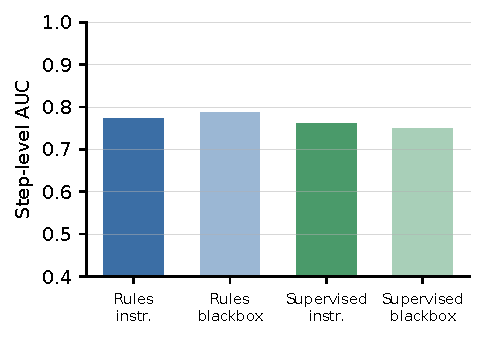
\includegraphics[width=0.62\linewidth]{figures/fig_gap.pdf}
\caption{Detectability gap. Step-level AUC is nearly unchanged when harness telemetry is hidden, but
type identification degrades---a monitor can see that something is wrong from error strings and
version counters without being able to say what it is.}
\label{fig:gap}
\end{figure}

Signal ablation (Table~\ref{tab:ablation}) shows error codes carry the most mass (removing them drops
event detection from 88\% to 64\%), with policy conformance and version staleness next at 74\%. A
monitor built purely on error codes is therefore not viable: the classes that dominate the harmful
set are not error-code failures.

\begin{table}[t]
\centering\small
\caption{Signal ablation for the rule-based detector: each row removes one
feature family and reports event-level detection rate. Error codes carry the most
mass; removing policy conformance or version/staleness loses a comparable share,
which is why a purely error-driven monitor is insufficient.}
\label{tab:ablation}
\begin{adjustbox}{max width=\textwidth}
\begin{tabular}{@{}lc@{}}
\toprule
Feature set & Detected (\%) \\
\midrule
full & 88.0 \\
$-$ error\_codes & 64.0 \\
$-$ version\_staleness & 74.0 \\
$-$ conflict & 80.0 \\
$-$ communication & 88.0 \\
$-$ progress & 88.0 \\
$-$ policy\_conformance & 74.0 \\
\bottomrule
\end{tabular}
\end{adjustbox}
\end{table}


\subsection{Recovery is class-dependent, and not in the order you would guess}

\begin{table}[t]
\centering\small
\caption{Recovery rate (\%) conditional on failure class. \emph{Det.} is the
rule-based detector's event recall for that class. Unrecoverable external errors
are reported as attempted repairs: the correct behaviour is containment, which is
scored separately (Sec.~\ref{sec:results}).}
\label{tab:bytype}
\begin{adjustbox}{max width=\textwidth}
\begin{tabular}{@{}lcccccc@{}}
\toprule
Failure class & No rec. & Retry & Rule & Model & Det. & $n$ \\
\midrule
invalid\_arguments & 0.0 & 0.0 & 95.9 & 73.4 & 100.0 & 169 \\
stale\_state & 0.0 & 0.0 & 76.3 & 68.4 & 86.8 & 76 \\
contradictory\_evidence & 0.0 & 0.0 & 96.2 & 96.2 & 100.0 & 158 \\
planning\_error & 0.0 & 0.0 & 40.9 & 41.8 & 80.0 & 110 \\
communication\_failure & 0.0 & 0.0 & 82.2 & 82.2 & 100.0 & 45 \\
objective\_drift & 0.0 & 0.0 & 52.2 & 23.1 & 97.8 & 134 \\
unrecoverable\_external\_error & 0.0 & 0.0 & 0.0 & 0.0 & 100.0 & 169 \\
\midrule
All & 0.0 & 0.0 & 60.9 & 51.3 & 95.9 & -- \\
\bottomrule
\end{tabular}
\end{adjustbox}
\end{table}


\begin{figure}[t]
\centering
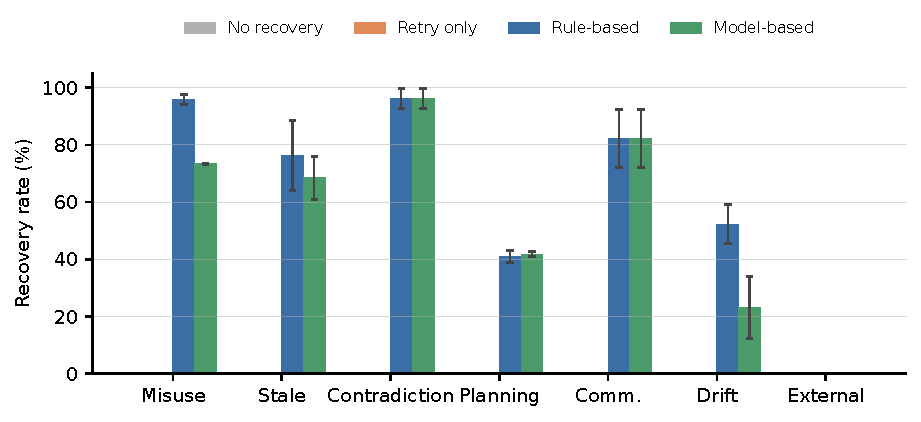
\includegraphics[width=\linewidth]{figures/fig_bytype.pdf}
\caption{Recovery by failure class with 95\% cluster-bootstrap intervals. Retries never help, and
the two classes that require an internal model of the task---planning error and objective
drift---are where recovery collapses.}
\label{fig:bytype}
\end{figure}

Table~\ref{tab:bytype} and Fig.~\ref{fig:bytype} are the core result. The ordering is not the
intuitive one. \emph{Contradictory evidence} is repaired 96\% of the time and \emph{misuse}
(mis-specified arguments) 96\%, despite the former being a ``latent'' class: both have a decisive,
cheap, local operator (re-read the authoritative source; re-derive the arguments). \emph{Planning
error} is repaired only 41\% and \emph{objective drift} 52\%, and those are the two classes whose
repair requires reconstructing what the task was supposed to accomplish. A replan that does not
recover the original objective simply produces a different wrong plan. This ordering is a
property of the repair operators, not of which selector chose them: the canonical mapping and
the learned ranker differ significantly after Holm correction in only
\HolmClassSignificant{} of \HolmClassTests{} classes---misuse and objective drift---and in both
the canonical mapping wins episode for episode (Table~\ref{tab:appendix_tests_class}). Where a
class has a cheap local operator, every selector finds it; where it does not, no selector does.

Two mechanical observations matter for anyone building on this. First, \emph{retry never works}:
retry-only recovers \RecRetry\% while spending more tool calls than the rule-based policy, because
retrying a deterministic tool reproduces the same failure and burns the budget. Second,
\emph{unrecoverable external errors are correctly contained but never recovered}, which is the right
answer; a policy that reports recovery on this class is either lying or was scored from self-report.

We also observe a systematic misattribution: in the accounting family the \texttt{close\_period}
precondition turns a silent objective-drift injection into a precondition error, so the monitor
labels it \emph{planning error} and applies the wrong operator. This is not a bug we patched away;
it is the phenomenon that makes drift hard---the surface signal points at the wrong class---and it is
part of why drift recovery sits at 52\%.

\subsection{Timing predicts recovery}

Detection \emph{speed} is not merely a diagnostic nicety. Splitting rule-based episodes by whether
the fault was detected at or before the injection step (i.e.\ before it could propagate) gives
\EarlyRec\% recovery over \EarlyN{} episodes versus \LateRec\% over \LateN{} late detections---a
\EarlyGap{} point gap. We report it as an association rather than a controlled effect, since
early-detectable faults are also the faults with the most visible signatures.

\begin{figure}[t]
\centering
\begin{subfigure}{0.48\linewidth}
\centering
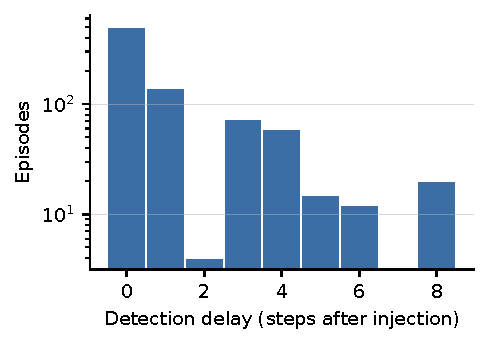
\includegraphics[width=\linewidth]{figures/fig_ttd.pdf}
\caption{Detection delay (rule-based).}
\end{subfigure}\hfill
\begin{subfigure}{0.48\linewidth}
\centering
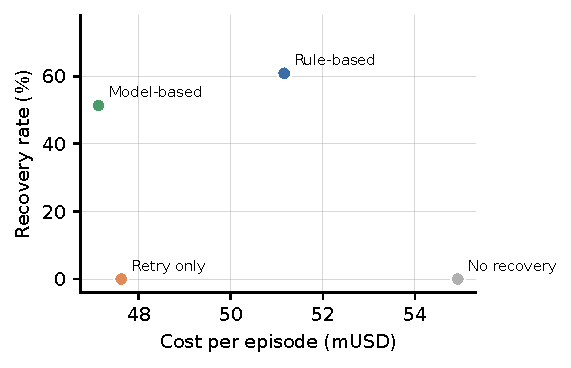
\includegraphics[width=\linewidth]{figures/fig_cost.pdf}
\caption{Cost vs.\ recovery.}
\end{subfigure}
\caption{Left: most detections land on the injection step, with a tail out to several steps. Right:
the cost-recovery frontier; the rule-based policy dominates on both axes, and ``no recovery'' is not
cheap because failed episodes run longer.}
\label{fig:ttd}
\end{figure}

\subsection{The learned ranker does not beat the canonical mapping}

\begin{table}[t]
\centering\small
\caption{Recovery performance by policy on the harmful-fault set
($n=\NumHarmful$ task--fault pairs per policy). Intervals are 95\% cluster
bootstrap over task templates. \emph{Tokens} is total model+tool tokens per
episode; \emph{USD} uses the fixed price sheet (Sec.~\ref{sec:cost}).}
\label{tab:main}
\begin{tabular}{@{}lccccccc@{}}
\toprule
Policy & Recovery \% [95\% CI] & Single & Multi & Detected \% & Calls & Tokens & USD \\
\midrule
No recovery & 0.0 [0.0, 0.0] & 0.0 & 0.0 & 0.0 & 14.34 & 17432 & 0.0549 \\
Retry only & 0.0 [0.0, 0.0] & 0.0 & 0.0 & 95.9 & 12.50 & 15134 & 0.0476 \\
Rule-based & 60.9 [57.9, 65.3] & 68.2 & 46.0 & 95.9 & 13.76 & 16074 & 0.0512 \\
Model-based & 51.3 [50.5, 51.7] & 59.4 & 35.1 & 99.4 & 13.00 & 14711 & 0.0471 \\
\bottomrule
\end{tabular}
\end{table}


Table~\ref{tab:main} is the headline comparison. No recovery: \RecNoRecovery\%. Retry only:
\RecRetry\%. Rule-based: \RecRules\%. Model-based: \RecModel\%. The learned ranker is a genuine
attempt---per-operator value models, calibrated features, a real candidate set---and it lands
\emph{below} the hand-written mapping. The diagnosis is off-policy confounding: the ranker only ever
sees the outcome of operators the rule-based policy chose, so for any state where the canonical
operator failed it has no counterfactual to learn from, and its containment head (which has the
fewest logged executions) fires on states where repair would have worked. We report this as a
boundary result: \emph{learning when to repair is not the bottleneck; learning what to repair
requires exploration the logged data does not contain.} The gap is not sampling noise: an exact
McNemar test on the \StatsPairs{} paired episodes rejects equality of the two policies
($b=\RuleVsModelB$ pairs recovered only by the canonical mapping, $c=\RuleVsModelC$ only by the
ranker, $p=\RuleVsModelP$), and it survives Holm correction over the \HolmPolicyTests{} policy
pairs ($p_{\text{Holm}}=\RuleVsModelPHolm$; Table~\ref{tab:appendix_tests_policy}).

\subsection{An LLM controller does not close the gap either}

\begin{table}[t]
\centering\small
\caption{Operator selection by a language model versus the canonical mapping, on identical
harmful pairs (\LLMPairs\ sampled harmful pairs, local model \texttt{\LLMModel}, detector held fixed at the rule monitor). The detector, the recovery programs and the grader are shared,
so the difference is attributable to which operator is applied.}
\label{tab:llm}
\begin{adjustbox}{max width=\textwidth}
\begin{tabular}{@{}lcccc@{}}
\toprule
Failure class & $n$ & Rule-based & LLM & $\Delta$ (pp) \\
\midrule
invalid\_arguments & 44 & 95.5 & 95.5 & +0.0 \\
stale\_state & 30 & 80.0 & 80.0 & +0.0 \\
contradictory\_evidence & 44 & 95.5 & 0.0 & -95.5 \\
planning\_error & 30 & 33.3 & 0.0 & -33.3 \\
communication\_failure & 11 & 81.8 & 0.0 & -81.8 \\
objective\_drift & 41 & 46.3 & 0.0 & -46.3 \\
unrecoverable\_external\_error & 40 & 0.0 & 0.0 & +0.0 \\
All & 240 & 60.8 & 27.5 & +33.3 \\
\bottomrule
\end{tabular}
\end{adjustbox}
\end{table}


The learned ranker is not the only selector we tried. To test whether the shortfall is a property of
our small model class rather than of the problem, we replace \emph{only} the operator-selection step
with a locally served 7B instruction model (\texttt{\LLMModel}, temperature 0, JSON-constrained
output). The detector, the nine recovery programs, the environments and the grader are unchanged, so
the comparison isolates the choice of operator; the prompt carries the detector's posterior and the
monitor feature vector plus the operator menu, and never the injected fault, its injection step, the
expected state or the grader's verdict. Replies are cached by prompt hash, so the arm replays exactly.
On \LLMPairs harmful pairs stratified by class \emph{and} family, the same pairs are replayed with
the canonical mapping: the LLM recovers \LLMRecovery\% against \LLMRuleRecovery\% for the rules, a
paired lead of \LLMPairedDelta{} points [\LLMPairedLo{}, \LLMPairedHi{}]. The interval is wide because
the cluster bootstrap resamples three templates; the point difference is not. An exact McNemar
test on the same \LLMPairs{} pairs rejects equality of the two selectors: the canonical mapping
recovers $b=\LLMMcNemarB$ pairs the LLM misses, and the LLM recovers $c=\LLMMcNemarC$ that the
mapping does not, $p=\LLMMcNemarP$. That test is pre-specified on its own 240-pair sample, so it
enters no Holm family (App.~\ref{app:tests}).

The pattern of failure is more informative than the aggregate. Where the class is \emph{surface} and
its name names its repair, the model reproduces the canonical mapping decision for decision---misuse
at \LLMMisuse\% (rules \LLMRuleMisuse\%), stale state at \LLMStale\% (rules \LLMRuleStale\%)---because
the menu entry (\texttt{revalidate\_args}, \texttt{refresh\_state}) is the obvious reading of the
alarm. Where the class is \emph{latent}---contradictory evidence, planning error, objective
drift---it falls back to \texttt{retry} (\LLMRetryPct\% of its \LLMDecisions{} decisions), which
repairs none of them, and on the unrecoverable class it retries instead of halting, containing
\LLMContainment\% of outages against \LLMRuleContainment\% for the rules. Reading a mapping that is
written down is within reach of a small model; \emph{inferring} one from evidence is not. The
\LLMCalls{} billed model calls cost nothing beyond the local server, so this is a capability result,
not a budget artefact.

\subsection{Held-out generalisation}

\begin{table}[t]
\centering\small
\caption{Held-out generalisation. \emph{test\_id} uses a seen task template
with an unseen environment configuration (higher concurrency); \emph{test\_ood}
uses an entirely held-out template. Detectors and rankers are fit on
\emph{train} only. Recovery rate (\%) with episode count in parentheses.}
\label{tab:split}
\begin{adjustbox}{max width=\textwidth}
\begin{tabular}{@{}lcccc@{}}
\toprule
Policy & Train & Dev & Test (ID) & Test (OOD) \\
\midrule
Rule-based & 60.7 (351) & 67.9 (109) & 62.4 (109) & 57.9 (292) \\
Model-based & 49.3 (351) & 52.3 (109) & 56.0 (109) & 51.7 (292) \\
\bottomrule
\end{tabular}
\end{adjustbox}
\end{table}


Generalisation is reassuringly flat (Table~\ref{tab:split}): the rule-based policy recovers 62.4\% on
the unseen configuration and 57.9\% on the unseen template, against 60.7\% on train, and the
model-based policy shows the same mild degradation. The detector and ranker never saw the held-out
template, so the taxonomy-based rules are doing real work rather than memorising schedules. The OOD
drop is concentrated in the migration family, where the held-out template adds a reconciliation
branch that the canonical operator program handles less directly.

\subsection{Single-agent versus multi-agent}

There is a consistent multi-agent penalty: \MultiRecovery\% recovery on multi-agent episodes versus
\SingleRecovery\% on single-agent episodes over the same fault classes. Part of this is structural
(multi-agent tasks have longer horizons and more state), but a specific mechanism is visible in the
coordination slice: \emph{communication failure} is repaired 82\% of the time by the rule-based
policy---the highest of any class---\emph{when} the bus can be re-synchronised, because the operator
(\texttt{resync\_message}) restores the receiving role's belief directly. Without it the failure is
invisible to the receiving agent: its belief is simply wrong, and no amount of re-reading its own
tools fixes a message it never got. Communication is therefore the class where multi-agent recovery
is qualitatively different from single-agent recovery rather than merely harder.

\subsection{The self-report gap}

Agents claim success in \ClaimedPct\% of evaluated episodes and are verified successful in
\VerifiedPct\%. \FalseClaimPct\% of episodes with a success claim failed the state check
(\FalseClaimN{} episodes). The gap is not uniform: it is largest in the migration family, where
``copied everything I was shown'' is true and ``everything was copied'' is false---a silent lost
update the agent has no way to observe. Any evaluator that reads the transcript, or asks the agent
whether it succeeded, would have scored those runs as wins. This is the single strongest argument for
state-verified scoring in this benchmark and we treat it as a finding, not a footnote.

\subsection{Cost}

\begin{table}[t]
\centering\small
\caption{Cost-aware outcomes under the fixed price sheet. \emph{USD/episode}
is the mean over all evaluated episodes; \emph{USD/recovered} is the total spend
divided by the number of recovered episodes, i.e.\ the amortised price of a
successful repair; \emph{USD/failed} is the mean spend on episodes that still
failed. Recovery is never free: detection and repair consume steps, tokens and
tool calls.}
\label{tab:cost}
\begin{adjustbox}{max width=\textwidth}
\begin{tabular}{@{}lccccc@{}}
\toprule
Policy & USD/episode & USD/recovered & USD/failed & Latency (ms) & Recovery \% \\
\midrule
No recovery & 0.0549 & -- & 0.0549 & 4927 & 0.0 \\
Retry only & 0.0476 & -- & 0.0476 & 4334 & 0.0 \\
Rule-based & 0.0512 & 0.0841 & 0.0341 & 4699 & 60.9 \\
Model-based & 0.0471 & 0.0918 & 0.0358 & 4452 & 51.3 \\
\bottomrule
\end{tabular}
\end{adjustbox}
\end{table}


Recovery is not free and ``no recovery'' is not cheap. Because failed episodes run to the end of the
procedure and retry, the no-recovery baseline spends \emph{more} than the rule-based policy in total
(Table~\ref{tab:cost}); repair truncates doom loops. The amortised view (USD per recovered episode)
is the fair comparison for a deployment: it prices the failures that were never repaired into the
cost of the ones that were. On that metric the rule-based policy is the only policy whose spend buys
recovery rather than activity.

\begin{figure}[t]
\centering
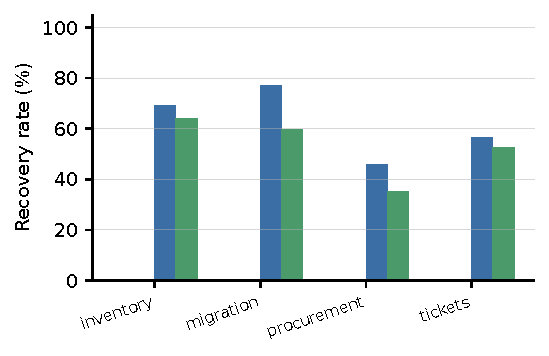
\includegraphics[width=0.6\linewidth]{figures/fig_family.pdf}
\caption{Recovery by environment family. The accounting family is hardest for every policy, and the
gap between rule-based and no-recovery is largest where state is auditable.}
\label{fig:family}
\end{figure}

\subsection{Provenance shift and long horizons}

\begin{table}[t]
\centering\small
\caption{Provenance shift: detections on faults produced by the agent's own
competence model rather than by the injection machinery ($n=\NaturalN$ episodes;
the rule-based policy and detector are used unchanged). Detected
\NaturalDetected\%, recovered \NaturalRecovery\%, class agreement
\NaturalAgreement\%.}
\label{tab:natural}
\begin{tabular}{@{}lc@{}}
\toprule
Agent-side failure class & Episodes \\
\midrule
invalid\_arguments & 12 \\
objective\_drift & 11 \\
planning\_error & 16 \\
\bottomrule
\end{tabular}
\end{table}


When failures are produced by the agent's own competence model instead of the injection machinery
(Table~\ref{tab:natural}), the unchanged rule detector finds \NaturalDetected\% of them and the
rule-based policy recovers \NaturalRecovery\%, with \NaturalAgreement\% agreement between detected
and true class. Event recall is lower than on injected faults---natural faults often have quieter
signatures---but conditional recovery is \emph{higher}, because natural faults tend to be local. The
taxonomy transfers; the operating point does not, which is exactly why a leaderboard must report
both.

\begin{table}[t]
\centering\small
\caption{Long-horizon slice (2--3$\times$ the steps of the main grid, with fully
observable state and success criteria). Recovery rate (\%) with episode count,
mean time-to-detection in steps, and mean tool calls.}
\label{tab:long}
\begin{tabular}{@{}lcccc@{}}
\toprule
Family & No recovery & Rule-based & TTD & Calls \\
\midrule
inventory & 0.0 (19) & 68.4 (19) & 1.21 & 22.3 \\
migration & 0.0 (16) & 75.0 (16) & 0.75 & 29.8 \\
procurement & 0.0 (25) & 52.0 (25) & 2.42 & 13.4 \\
tickets & 22.2 (18) & 66.7 (18) & 0.29 & 18.4 \\
\bottomrule
\end{tabular}
\end{table}


Long-horizon tasks (Table~\ref{tab:long}) confirm the pattern at 2--3$\times$ the step count with
fully observable state: detection still lands within about a step of injection for rules, but
recovery rates fall and downstream impact grows, because there are more steps after the fault for the
damage to reach.

\section{Discussion}\label{sec:discussion}

\paragraph{Which failure signals predict successful recovery?} Three, in descending order of
strength. \emph{Class} is the dominant predictor, and specifically whether the class has a cheap
local operator: misuse and contradictory evidence are repaired at roughly 96\%, while planning error
(41\%) and objective drift (52\%) are not, because their repair requires reconstructing intent that
is not present in any observation. \emph{Timing} is second: detection before propagation is worth
roughly \EarlyGap{} points of recovery within the same policy. \emph{Signal type} is third and is
what makes class prediction possible at all---error codes alone detect 64\% of harmful faults, and
adding staleness, conflict, policy-conformance and progress features recovers the rest. Notably, the
predictors that matter are \emph{structural}, not stylistic: token counts, latency and retry counts
carry almost no information about whether a repair will succeed.

\paragraph{Repair has a ceiling that detection cannot lift.} The most useful negative result here is
the shape of the failure: detection AUC near 0.8 with recovery at 61\%. Even a perfect detector would
not close the gap, because the remaining failures are class-confusion and operator-locality problems.
This reframes the research agenda. Work that improves monitors (better step-level classifiers,
process reward models, LLM critics) attacks the smaller half of the problem. The larger half is
\emph{repair operators}: re-anchoring an objective, or replanning from a damaged belief state, is a
different capability from noticing that something is wrong, and it is where the numbers are low.

The LLM-controller experiment points the same way. The classes it repairs as well as the rules are
exactly the ones whose operator is named after their symptom (misuse, staleness); the classes whose
repair requires reconstructing intent collapse to retries. Operator locality, not signal visibility,
is again what separates repair from detection.

\paragraph{The learned-policy result is a data problem, not a modelling problem.} Our ranker failed
to beat the canonical mapping. We could have hidden this by tuning the candidate set, and we chose
not to, because the diagnosis is the interesting part: recovery policy learning from logged
trajectories is an off-policy problem, and the logging policy never takes the actions we need to
evaluate. Fixing it requires exploration in the sandbox (a small amount of deliberate operator
randomisation during data collection) rather than a better model class. That is a concrete,
actionable design for the next version of the benchmark, and it is exactly the kind of finding a
benchmark should produce about itself.

\paragraph{Why state-verified scoring is not optional.} The self-report gap (\ClaimedPct\% claimed
vs \VerifiedPct\% verified) is the clearest practical lesson. It is not that agents lie; it is that
the information needed to know they failed is not in the transcript. In the migration family a lost
update is invisible to an agent that only sees what it wrote. Any evaluation based on transcript
inspection, LLM-judge grading, or self-reported completion is measuring confidence, not reliability.

\paragraph{What a leaderboard should and should not reward.} \arb{} is designed so that a system
cannot win by being conservative (containment is scored separately and counts as failure to
recover), by being verbose (tokens are costed), by retrying (retry-only is a baseline at 0\%), or by
claiming success (claims are ignored). What it rewards is conditional recovery at bounded cost with
containment on the unrecoverable class. Because the harmful set is fixed by the screen, every
entrant is scored on the same faults, which is what makes cross-system comparison meaningful.

\paragraph{Limitations and threats to validity}\label{sec:limits}

\begin{itemize}
\item \textbf{Simulation.} Every environment is a deterministic Python world. Real tools are
partially observable, non-deterministic, and slow; real failures are heavily correlated with load,
version skew and human behaviour. \arb{} measures \emph{relative} reliability under controlled
faults. It cannot tell you an agent's production recovery rate, and a system that ranks first here
may not rank first in deployment.
\item \textbf{Scripted agents, LLM controller.} The agents that execute tasks are scripted workflow
executors with a known SOP. They are a strong control (deterministic, belief-grounded, replayable) and
a narrow sample of agent behaviour. We supplement them with a local 7B model used as the
\emph{recovery controller} (\LLMRecovery\% versus \LLMRuleRecovery\% for the rules on the same
pairs), which is a capability result about operator selection, not about planning. A frontier model
driving both the plan and the repair is still not evaluated, so the numbers characterise the
\emph{harness and the fault set} rather than any deployed model.
\item \textbf{Harm screening induces selection.} Excluding inert faults biases the retained set
toward faults with large downstream reach, which inflates apparent harmfulness and may make
recovery look harder than it is for the average injection. We chose this because the alternative---a
denominator containing faults that no monitor could be blamed for---makes recall uninterpretable.
\item \textbf{Cluster bootstrap over templates.} With a few dozen templates the bootstrap is
coarse; intervals should be read as indicating order of magnitude, not third-decimal precision.
\item \textbf{Single lab, single author.} Labels are defined by an injection program, which removes
annotator disagreement but also removes the chance to discover classes we did not think of. Natural
faults partially mitigate this, and their class agreement (\NaturalAgreement\%) is encouraging, but
the taxonomy is not exhaustive.
\item \textbf{Cost model.} The price sheet is a fixed artefact; USD figures are a transparent
normalisation, not a market forecast.
\end{itemize}

\paragraph{Ethics and safety.} Fault injection is confined to sandboxed, non-production
environments with no external side effects; no real refunds, orders or migrations occur. The
benchmark's emphasis on containment is deliberate: an agent that stops mutating when it does not
understand the world is safer, and scoring containment separately prevents the benchmark from
rewarding agents that push through uncertainty. Releasing a recovery policy that is only evaluated
in sandbox is a real risk---it invites deployment outside the tested boundary---so the released
ranker is packaged with an explicit out-of-scope statement, and the leaderboard protocol requires
sandbox evaluation of any submitted policy. We do not release attack tooling: the injection
programs perturb only the benchmark's own environments.

\section{Release and Leaderboard Protocol}\label{sec:release}

\subsection{Artifacts}

\begin{table}[h]
\centering\small
\caption{Release contents. All artefacts are produced by the pinned commit; the dataset and models
are published on the Hugging Face Hub and mirrored in the repository that builds this PDF.}
\label{tab:release}
\footnotesize
\setlength{\tabcolsep}{4pt}
\begin{adjustbox}{max width=\textwidth}
\begin{tabular}{@{}lll@{}}
\toprule
Artefact & Path & Purpose \\
\midrule
Dataset (episodes) & \texttt{data/arb\_dataset.jsonl} & one row per (task, fault, policy) episode \\
Dataset (steps) & \texttt{data/arb\_steps.jsonl} & one row per step, with state and labels \\
Mini split & \texttt{data/arb\_mini.jsonl} & 120-episode smoke subset \\
Harness & \texttt{arb/} & environments, injection, monitors, policies, metrics \\
Detector & \texttt{models/detector.json} & supervised step classifier + calibration \\
Ranker & \texttt{models/recovery\_ranker.json} & per-operator value models \\
Configs & \texttt{configs/*.yaml} & exact grids for main, long-horizon, blackbox runs \\
Scripts & \texttt{scripts/} & \texttt{run\_experiments}, \texttt{build\_dataset}, \texttt{push\_to\_hub} \\
Cards & \texttt{docs/} & dataset card, model card, taxonomy, protocol \\
Paper & \texttt{paper/main.pdf} & this document, with generated tables \\
\bottomrule
\end{tabular}
\end{adjustbox}
\end{table}

\subsection{Leaderboard protocol}

The protocol is fixed so that entries are comparable across time.

\begin{enumerate}[leftmargin=1.4em]
\item \textbf{Pinned versions.} An entry names a tag of this repository (harness), the dataset
revision hash, and the price-sheet version. Scores are only comparable within a tag.
\item \textbf{Fixed splits.} Fit on \emph{train} only. \emph{Dev} may be used for thresholds and
hyper-parameters. \emph{Test-id} and \emph{test-ood} are reported, never fitted. Submitting a system
that was tuned on test-ood is grounds for removal.
\item \textbf{Fixed denominators.} The harmful set is defined by the frozen screen (no-recovery runs,
seed 0--2). Every entrant is scored on the same pairs. Adding faults requires a new dataset
revision, not a new scoreboard.
\item \textbf{Five required numbers.} Recovery rate with 95\% cluster-bootstrap interval; detection
precision/recall/F1/AUC (step-level) in both monitor regimes; USD per recovered episode; containment
rate on unrecoverable faults; and the self-report gap (claimed minus verified).
\item \textbf{Verification.} Success is read from world state only. A submission must include the
grader-verified outcomes for its episodes; claims without state dumps are not scored.
\item \textbf{No oracle access.} A monitor may not read the fault plan, the injection step, expected
state, or the grader verdict. Instrumented monitoring may read harness telemetry flags; blackbox
entries may not, and both columns are published.
\item \textbf{Compute disclosure.} Entries report training cost and inference cost per episode.
\item \textbf{Containment is not recovery.} Escalating on a recoverable fault scores zero recovery.
Stopping on an unrecoverable fault scores full containment and zero recovery.
\end{enumerate}

\subsection{Reproduction}

Two commands reproduce every number, table and figure in this paper from a clean checkout:
\begin{Verbatim}[fontsize=\footnotesize]
pip install -e .
python scripts/run_experiments.py --config configs/main.yaml
python paper/analysis.py && latexmk -pdf paper/main.tex
\end{Verbatim}
\texttt{scripts/}\allowbreak\texttt{build\_dataset.py} regenerates the released JSONL from the
harness, and \texttt{scripts/}\allowbreak\texttt{push\_to\_hub.py} publishes it; the latter
requires the user's Hugging Face token and is never run automatically. Determinism is checked by \texttt{tests/run\_tests.py}, which asserts
byte-identical trajectories for a fixed seed and the invariants the harness depends on (faults are
exercised, success is state-verified, detection is never counted before injection).

\subsection{Code and data availability}

Everything needed to check a number in this paper is public and versioned. The dataset
(episodes, steps, mini split and the \texttt{llm} controller arm) is archived at
\url{https://huggingface.co/datasets/fahadhafeezofficial/agent-recovery-bench}; the fitted
detector, the recovery ranker and the LLM-arm result file are archived at
\url{https://huggingface.co/fahadhafeezofficial/agent-recovery-bench-models}. Both carry a
revision hash, and a result is only comparable to another produced under the same harness tag
(\texttt{arb-1.0.0}) and price sheet (\texttt{arb-price-2026.11}).

The harness, the reference agents, the evaluator, the experiment grid and the analysis script
that emits every table and figure are released under the MIT licence (\texttt{LICENSE};
\texttt{pyproject.toml} declares the same licence) at
\url{https://github.com/Fahad-Hafeez/agent-recovery-bench}, tagged \texttt{arb-1.0.0}, which is the version this paper was built from, and citable via
\texttt{CITATION.cff}. The archive
includes \texttt{results/} and the generated tables, so \texttt{pdflatex} rebuilds this PDF
from a clean checkout without re-running the 4-minute grid; re-running
\texttt{paper/analysis.py} must leave those files byte-identical, which is the check that the
PDF has not drifted. \texttt{data/} is regenerable with \texttt{scripts/build\_dataset.py}
and is not duplicated in the source archive. No credential is needed to reproduce any number;
the only authenticated step is publishing to the Hub (	exttt{scripts/push\_to\_hub.py}), which
reads a token from the environment and is never run automatically. The snapshot this PDF was
built from is also downloadable as a tarball:
\url{https://github.com/Fahad-Hafeez/agent-recovery-bench/archive/refs/tags/arb-1.0.0.tar.gz}

\subsection{Extending the benchmark}

New environments must implement the four-method contract (\texttt{invoke},
\texttt{authoritative\_step}, \texttt{resync\_step}, \texttt{repair\_args}) and declare which fault
classes they support; the injection programs are class-level and family-agnostic, so a new family
immediately inherits all seven classes. New failure classes require a program, a canonical operator,
and a detectability label---if a class has no operator that repairs it in at least one family, it
belongs in the contain-only bucket alongside unrecoverable external error.

\appendix

\section{Full tables}\label{app:full}

Every number in this appendix is generated by the analysis script from the three result
artifacts the experiments write; none is typed by hand. Point estimates here are the same
values reported in the main text, so a reader can check one against the other.

\subsection{Recovery by failure class and policy}

\begin{table}[!ht]
\centering\scriptsize
\setlength{\tabcolsep}{4pt}
\caption{Recovery rate (\% of harmful pairs) by failure class with 95\% cluster-bootstrap intervals over task templates. \emph{Det.} is the rule monitor's event recall for that class. The unrecoverable class is reported as attempted repair; containment is scored separately.}
\label{tab:appendix_class}
\begin{adjustbox}{max width=\textwidth}
\begin{tabular}{@{}lrccccr@{}}
\toprule
Failure class & $n$ & No recovery & Retry only & Rule-based & Model-based & Det. \\
\midrule
invalid\_arguments & 169 & 0.0 [0.0, 0.0] & 0.0 [0.0, 0.0] & 95.9 [94.6, 98.2] & 73.4 [73.2, 73.7] & 100.0 \\
stale\_state & 76 & 0.0 [0.0, 0.0] & 0.0 [0.0, 0.0] & 76.3 [65.0, 89.3] & 68.4 [60.0, 75.0] & 86.8 \\
contradictory\_evidence & 158 & 0.0 [0.0, 0.0] & 0.0 [0.0, 0.0] & 96.2 [92.7, 100.0] & 96.2 [92.7, 100.0] & 100.0 \\
planning\_error & 110 & 0.0 [0.0, 0.0] & 0.0 [0.0, 0.0] & 40.9 [38.5, 42.9] & 41.8 [41.0, 42.9] & 80.0 \\
communication\_failure & 45 & 0.0 [0.0, 0.0] & 0.0 [0.0, 0.0] & 82.2 [73.3, 93.3] & 82.2 [73.3, 93.3] & 100.0 \\
objective\_drift & 134 & 0.0 [0.0, 0.0] & 0.0 [0.0, 0.0] & 52.2 [44.2, 57.8] & 23.1 [8.9, 30.4] & 97.8 \\
unrecoverable\_external\_error & 169 & 0.0 [0.0, 0.0] & 0.0 [0.0, 0.0] & 0.0 [0.0, 0.0] & 0.0 [0.0, 0.0] & 100.0 \\
\bottomrule
\end{tabular}
\end{adjustbox}
\end{table}


\subsection{Recovery by environment family}

\begin{table}[!ht]
\centering\scriptsize
\setlength{\tabcolsep}{4pt}
\caption{Recovery rate (\%) by environment family and policy with 95\% cluster-bootstrap intervals. The accounting family is hardest for every policy; the gap between rule-based and no recovery is largest where state is auditable.}
\label{tab:appendix_family}
\begin{tabular}{@{}lrcccc@{}}
\toprule
Family & $n$ & No recovery & Retry only & Rule-based & Model-based \\
\midrule
inventory & 217 & 0.0 [0.0, 0.0] & 0.0 [0.0, 0.0] & 69.1 [65.8, 73.6] & 64.1 [61.6, 68.1] \\
migration & 196 & 0.0 [0.0, 0.0] & 0.0 [0.0, 0.0] & 77.0 [75.0, 78.6] & 59.7 [56.7, 62.9] \\
procurement & 285 & 0.0 [0.0, 0.0] & 0.0 [0.0, 0.0] & 46.0 [40.0, 55.7] & 35.1 [30.0, 41.2] \\
tickets & 163 & 0.0 [0.0, 0.0] & 0.0 [0.0, 0.0] & 56.4 [49.0, 64.4] & 52.8 [47.5, 56.9] \\
\bottomrule
\end{tabular}
\end{table}


\subsection{Step-level detection with intervals}\label{app:detection}

\begin{table}[!ht]
\centering\scriptsize
\setlength{\tabcolsep}{4pt}
\caption{Step-level detection with 95\% cluster-bootstrap intervals over task templates (\DetectionClusters{} clusters for the instrumented arms). Precision, recall, F1 and type accuracy are percentages; AUC is a proportion. The intervals are wide because the cluster bootstrap resamples whole templates, and three templates cannot pin a step-level rate to better than a few points. They describe the \emph{published} run: \texttt{scripts/detection\_intervals.py} replays the detector arm and aborts unless every point estimate reproduces \texttt{report\_main.json} exactly.}
\label{tab:detection_ci}
\begin{adjustbox}{max width=\textwidth}
\begin{tabular}{@{}llccccccc@{}}
\toprule
Detector & Monitor & Precision & Recall & F1 & AUC & Type & Steps & Cl. \\
\midrule
Rules & instr. & 66.9 [66.2, 68.1] & 41.9 [40.1, 44.8] & 51.5 [50.0, 53.4] & 0.772 [0.749, 0.789] & 34.6 [33.6, 36.2] & 24,175 & 3 \\
Rules & blackbox & 86.7 [85.7, 87.7] & 32.0 [31.7, 32.3] & 46.7 [46.5, 46.9] & 0.787 [0.759, 0.822] & 22.1 [21.7, 22.6] & 1,094 & 2 \\
Supervised & instr. & 48.8 [42.4, 54.5] & 86.2 [84.7, 89.1] & 62.3 [56.5, 67.6] & 0.762 [0.753, 0.770] & 51.6 [49.3, 53.8] & 11,193 & 3 \\
Supervised & blackbox & 46.0 [43.7, 48.7] & 81.0 [80.5, 81.5] & 58.7 [56.7, 60.9] & 0.750 [0.747, 0.752] & 39.9 [37.4, 42.7] & 1,060 & 2 \\
\bottomrule
\end{tabular}
\end{adjustbox}
\end{table}


\begin{table}[!ht]
\centering\scriptsize
\setlength{\tabcolsep}{4pt}
\caption{Step-level detection by split, per detector and monitor regime. Detection neither improves nor collapses out of distribution, which is what a taxonomy-defined monitor should show: the rules encode the signal, not the fault schedule.}
\label{tab:appendix_split_det}
\begin{adjustbox}{max width=\textwidth}
\begin{tabular}{@{}llrcc@{}}
\toprule
Arm & Split & Steps & AUC & Firing rate (\%) \\
\midrule
rules / instrumented & train & 10,186 & 0.755 & 20.4 \\
rules / instrumented & dev & 2,672 & 0.758 & 27.1 \\
rules / instrumented & test-id & 2,703 & 0.779 & 27.3 \\
rules / instrumented & test-ood & 8,614 & 0.789 & 21.5 \\
rules / blackbox & test-id & 491 & 0.822 & 13.2 \\
rules / blackbox & test-ood & 603 & 0.759 & 11.6 \\
supervised / instrumented & train & 4,170 & 0.745 & 67.8 \\
supervised / instrumented & dev & 1,426 & 0.774 & 58.7 \\
supervised / instrumented & test-id & 1,324 & 0.762 & 65.1 \\
supervised / instrumented & test-ood & 4,273 & 0.770 & 63.7 \\
supervised / blackbox & test-id & 487 & 0.752 & 61.2 \\
supervised / blackbox & test-ood & 573 & 0.747 & 61.1 \\
\bottomrule
\end{tabular}
\end{adjustbox}
\end{table}


\section{Paired significance tests}\label{app:tests}

The main text reports cluster-bootstrap intervals, which answer ``how large is the
difference''. This appendix adds the complementary question---``is a difference present at
all''---with an exact McNemar test on the aligned episode-level outcomes of two policies,
followed by a Holm--Bonferroni step-down correction within each family of tests. Only
discordant pairs carry information: $b$ is the number of episodes the first system recovered
and the second did not, $c$ the reverse. The two-sided $p$-value is an exact binomial test on
$b+c$ pairs at $p=0.5$; no chi-square approximation is used, and no $t$- or Wilcoxon test is
appropriate because the outcome is a paired bit.

Three families are corrected separately: the \HolmPolicyTests{} policy pairs, the
\HolmClassTests{} per-class rule-versus-ranker contrasts and the \HolmFamilyTests{}
per-family contrasts. Correcting across all of them at once would test a question nobody
asked. The LLM-controller arm is a case of its own: its 240 pairs are a different denominator,
drawn from the same grid but scored against a different controller, so it gets a single
pre-specified test rather than membership of a family. The canonical mapping recovers
$b=\LLMMcNemarB$ of those pairs and the LLM $c=\LLMMcNemarC$, an exact McNemar $p=\LLMMcNemarP$;
no correction applies because there is one test and it was not chosen after seeing the outcome.
\texttt{scripts/llm\_paired\_test.py} recomputes it from the released export, aborting unless the
joined outcomes reproduce \texttt{results/llm\_agent.json} exactly.

\begin{table}[!ht]
\centering\scriptsize
\setlength{\tabcolsep}{4pt}
\caption{Exact McNemar tests over the 861 harmful pairs: all six policy contrasts, Holm-corrected across the six. $b$ counts episodes the first system recovered and the second did not, $c$ the reverse. The canonical mapping beats the learned ranker: $b=104$ against $c=22$.}
\label{tab:appendix_tests_policy}
\begin{tabular}{@{}lrrrcc@{}}
\toprule
Comparison & Pairs & $b$ & $c$ & $p$ & $p_{\text{Holm}}$ \\
\midrule
No recovery vs Retry only & 861 & 0 & 0 & 1.000 & 1.000 \\
No recovery vs Rule-based & 861 & 0 & 524 & \ensuremath{<}0.001 & \ensuremath{<}0.001 \\
No recovery vs Model-based & 861 & 0 & 442 & \ensuremath{<}0.001 & \ensuremath{<}0.001 \\
Retry only vs Rule-based & 861 & 0 & 524 & \ensuremath{<}0.001 & \ensuremath{<}0.001 \\
Retry only vs Model-based & 861 & 0 & 442 & \ensuremath{<}0.001 & \ensuremath{<}0.001 \\
Rule-based vs Model-based & 861 & 104 & 22 & \ensuremath{<}0.001 & \ensuremath{<}0.001 \\
\bottomrule
\end{tabular}
\end{table}


\begin{table}[!ht]
\centering\scriptsize
\setlength{\tabcolsep}{4pt}
\caption{Per-class McNemar tests, rule-based versus model-based, Holm-corrected across the seven classes (significant in 2 of 7). Where the two policies differ at all, they differ in favour of the canonical mapping; the remaining classes agree closely, which is the claim the class table makes: repair depends on the operator, not the selector.}
\label{tab:appendix_tests_class}
\begin{adjustbox}{max width=\textwidth}
\begin{tabular}{@{}lrrrcc@{}}
\toprule
Failure class & Pairs & $b$ (rules) & $c$ (ranker) & $p$ & $p_{\text{Holm}}$ \\
\midrule
invalid\_arguments & 169 & 38 & 0 & \ensuremath{<}0.001 & \ensuremath{<}0.001 \\
stale\_state & 76 & 17 & 11 & 0.345 & 1.000 \\
contradictory\_evidence & 158 & 0 & 0 & 1.000 & 1.000 \\
planning\_error & 110 & 0 & 1 & 1.000 & 1.000 \\
communication\_failure & 45 & 0 & 0 & 1.000 & 1.000 \\
objective\_drift & 134 & 49 & 10 & \ensuremath{<}0.001 & \ensuremath{<}0.001 \\
unrecoverable\_external\_error & 169 & 0 & 0 & 1.000 & 1.000 \\
\bottomrule
\end{tabular}
\end{adjustbox}
\end{table}


\begin{table}[!ht]
\centering\scriptsize
\setlength{\tabcolsep}{4pt}
\caption{Per-family McNemar tests, rule-based versus model-based, Holm-corrected across the four families (significant in 3 of 4).}
\label{tab:appendix_tests_family}
\begin{tabular}{@{}lrrrcc@{}}
\toprule
Family & Pairs & $b$ (rules) & $c$ (ranker) & $p$ & $p_{\text{Holm}}$ \\
\midrule
inventory & 217 & 12 & 1 & 0.003 & 0.007 \\
migration & 196 & 34 & 0 & \ensuremath{<}0.001 & \ensuremath{<}0.001 \\
procurement & 285 & 42 & 11 & \ensuremath{<}0.001 & \ensuremath{<}0.001 \\
tickets & 163 & 16 & 10 & 0.327 & 0.327 \\
\bottomrule
\end{tabular}
\end{table}


\section{Grid, hyper-parameters and cost model}\label{app:grid}

\textbf{Grid.} \NumPairs{} (task, fault) pairs from four families $\times$ three templates
$\times$ five configurations $\times$ three seeds, of which \NumHarmful{} are harmful after
the screen; \NumEpisodes{} episodes are evaluated in total, including the natural-fault,
long-horizon, blackbox and ablation slices. Templates A/B and configurations
\texttt{cfg1}--\texttt{cfg3} are \emph{train}; \texttt{cfg5} is \emph{dev}; \texttt{cfg6} is an
unseen configuration (\emph{test-id}); template C is entirely held out (\emph{test-ood}).
Fault schedules are drawn per task from a seeded RNG, so memorising a schedule is not a
viable strategy.

\textbf{Detectors.} The rule monitor is 13 hand-written rules over the 19 monitor features; it
has no fitted parameters. The supervised detector is a multinomial logistic regression (8
classes including \emph{none}, L2 $=2\times10^{-3}$, learning rate $0.15$, 900 epochs, class
balancing) fit on \DetTrainRows{} training steps; its decision threshold ($\tau=\SupThreshold$)
is swept on \emph{dev} to maximise F1 and never on a reporting split. The recovery ranker is a
set of per-operator logistic value models fit on deliberate decisions from the rule-based
policy on \emph{train}, with operators seen fewer than 25 times excluded from the candidate set.

\textbf{Intervals.} 95\% cluster bootstrap resampling whole task templates (2000 resamples for
the reported tables), a paired bootstrap for policy differences, and Wilson intervals for
single proportions. Because the grid has only three templates, template-clustered intervals are
coarse by construction; they are reported rather than replaced by episode-level intervals,
which would pretend episodes are independent draws.

\textbf{Cost.} USD comes from the fixed price sheet \texttt{arb-price-2026.11} with
deterministic per-step jitter seeded by the episode id, so a cost figure is reproducible
rather than sampled. The sheet is a transparent normalisation of token, tool-call and latency
prices, not a market forecast.

\begin{sloppypar}
\textbf{Reproduction.} \texttt{python scripts/run\_experiments.py --preset main} writes the
report and the episode table; \texttt{python scripts/detection\_intervals.py} replays the
detector arm and writes the interval artifact, aborting if it cannot reproduce the report;
\texttt{python scripts/llm\_paired\_test.py} recomputes the LLM arm's paired test from the
released export, aborting unless it reproduces the scored aggregates;
\texttt{python paper/analysis.py} writes every table, figure and macro here; two
\texttt{pdflatex} passes and one \texttt{bibtex} pass rebuild this PDF. The harness is tag
\texttt{arb-1.0.1}, and the dataset revision must be pinned with it for any comparison.
\end{sloppypar}

\section{The controller prompt}\label{app:prompt}

The LLM-controller arm replaces only the operator-selection step. The prompt below is emitted
verbatim from \texttt{arb/agents/llm.py}, so the no-oracle claim can be checked without reading
code: it carries the detector's posterior over classes, the monitor feature vector and the
operator menu, and it contains no field identifying the injected fault, its injection step,
the expected state or the grader's verdict. The step number it quotes is the step at which the
alarm fired, not the step at which the fault was injected.

% Auto-generated by paper/analysis.py -- do not edit.
{\footnotesize
\begin{verbatim}
You are the recovery controller of a tool-using agent. A monitor has raised an
    alarm after a tool call. Choose exactly one recovery operator from the
    menu: the one whose precondition matches the evidence. Prefer the least
    disruptive operator that addresses the cause; do not invent operators.
    Reply with JSON only: {"action": "<operator>", "confidence": <0-1>,
    "reason": "<10 words max>"}.

% ---- user message ----
Alarm at step 7. Retries used 0/2.
Failure posterior: stale_state=0.710, planning_error=0.120,
    objective_drift=0.090, contradictory_evidence=0.080
Monitor evidence: version_lag=2.00, stale_flag=1.00, _score=0.66,
    step_pressure=0.40
Operators:
- continue: alarm is a false positive; keep executing the plan unchanged
- retry: re-issue the identical call once (transient transport error only)
- revalidate_args: repair the call's arguments against the tool schema, then
    re-issue
- refresh_state: re-read the object being mutated so the write uses current
    state
- re_read_authoritative: re-read the authoritative source and adopt its value
    over other observations
- replan: discard the remaining steps and recompute the plan from current
    state
- resync_message: re-send or re-read the inter-agent message so the recipient
    acts on the sender's plan
- reanchor_objective: restore the stated objective and recompute the plan
    under it
- escalate_abort: halt cleanly with no further mutations and escalate to a
    human
Choose one operator.
\end{verbatim}
}



\bibliographystyle{plain}
\begin{thebibliography}{99}\small

\bibitem{yao2023react} S. Yao, J. Zhao, D. Yu, N. Du, I. Shafran, K. Narasimhan, Y. Cao.
ReAct: Synergizing reasoning and acting in language models. \emph{ICLR}, 2023.

\bibitem{shinn2023reflexion} N. Shinn, F. Cassano, A. Gopinath, K. Narasimhan, S. Yao.
Reflexion: Language agents with verbal reinforcement learning. \emph{NeurIPS}, 2023.

\bibitem{yao2024taubench} S. Yao, N. Shinn, P. Razavi, K. Narasimhan.
$\tau$-bench: A benchmark for tool-agent-user interaction in real-world domains.
\emph{ICLR}, 2025. arXiv:2406.12045.

\bibitem{taubench2} V. Barres et al. $\tau^2$-bench: Evaluating conversational agents in a
dual-control environment. arXiv:2506.07982, 2025.

\bibitem{zhang2025whowhen} S. Zhang, M. Zhang, J. Ma, Y. Yang, Y. Zhang, Z. Liu, C. Yang.
Which agent causes task failures? Attributing failures in multi-agent systems.
\emph{ICML}, 2025. arXiv:2505.00212.

\bibitem{cemri2025mast} M. Cemri, M. Pan, S. Yang, L. Agrawal, B. Chopra, R. Tiwari, K. Keutzer,
A. Parameswaran, D. Klein, A. Ramakrishnan, S. Sinha, K. Narasimhan.
Why do multi-agent LLM systems fail? \emph{NeurIPS Datasets and Benchmarks}, 2025.
arXiv:2503.13657.

\bibitem{suzgun2025failuretaxonomy} M. Suzgun, M. Yuksekgonul, F. Bianchi, D. Jurafsky, J. Zou.
Measuring and mitigating thinking failures in reasoning models. arXiv:2506.12179, 2025.

\bibitem{hsueh1997fault} M.-C. Hsueh, T. K. Tsai, R. K. Iyer. Fault injection techniques and
tools. \emph{IEEE Computer}, 30(4):75--82, 1997.

\bibitem{scully2015fault} Z. Scully, G. Cottrell, M. Egele. Fault injection for software
reliability. \emph{IEEE Software}, 32(4), 2015.

\bibitem{lightstone2004chaos} S. Lightstone. Chaos engineering for distributed systems.
\emph{ACM Queue}, 2004.

\bibitem{basiri2016chaos} A. Basiri, N. Behnam, R. de Rooij, L. Hochstein, L. Kosewski,
J. Reynolds, C. Rosenthal. Chaos engineering. \emph{IEEE Software}, 33(3):35--41, 2016.

\bibitem{amodei2016concrete} D. Amodei, C. Olah, J. Steinhardt, P. Christiano, J. Schulman,
D. Man\'e. Concrete problems in AI safety. arXiv:1606.06565, 2016.

\bibitem{lightman2023prm} H. Lightman, V. Kosaraju, Y. Burda, H. Edwards, B. Baker, T. Lee,
J. Leike, J. Schulman, I. Sutskever, K. Cobbe. Let's verify step by step. \emph{ICLR}, 2024.

\bibitem{uesato2022safety} J. Uesato, N. Kushman, R. Kumar, F. Song, N. Siegel, L. Wang,
A. Creswell, G. Irving, I. Higgins. Solving math word problems with process- and outcome-based
feedback. arXiv:2211.14275, 2022.

\bibitem{wang2024survey} L. Wang, C. Ma, X. Feng, Z. Zhang, H. Yang, J. Zhang, Z. Chen, J. Tang,
X. Chen, Y. Lin, W. X. Zhao, Z. Wei, J.-R. Wen. A survey on large language model based autonomous
agents. \emph{Frontiers of Computer Science}, 18(6), 2024.

\bibitem{kim2023agents} Y. Kim, C. Kim, J. Lee, S. Lee, H. Lim. A survey on LLM-based agent
evaluation: from components to systems. \emph{EMNLP Findings}, 2024.

\bibitem{liu2023agentbench} X. Liu, H. Yu, H. Zhang, Y. Xu, X. Lei, H. Lai, Y. Gu, H. Ding,
K. Men, K. Yang, S. Zhang, X. Deng, A. Zeng, Z. Du, C. Zhang, S. Shen, T. Zhang, Y. Su, H. Sun,
M. Huang, Y. Dong, J. Tang. AgentBench: Evaluating LLMs as agents. \emph{ICLR}, 2024.

\bibitem{mialon2023gaia} G. Mialon, C. Fourrier, C. Swift, T. Wolf, Y. LeCun, T. Scialom.
GAIA: A benchmark for general AI assistants. \emph{ICLR}, 2024.

\bibitem{zhou2023webarena} S. Zhou, F. F. Xu, H. Zhu, X. Zhou, R. Lo, A. Sridhar, X. Cheng,
T. Ou, Y. Bisk, D. Fried, U. Alon, G. Neubig. WebArena: A realistic web environment for building
autonomous agents. \emph{ICLR}, 2024.

\bibitem{deng2023mind2web} X. Deng, Y. Gu, B. Zheng, S. Chen, S. Stevens, B. Wang, H. Sun,
Y. Su. Mind2Web: Towards a generalist agent for the web. \emph{NeurIPS}, 2023.

\bibitem{patil2023gorilla} S. G. Patil, T. Zhang, X. Wang, J. E. Gonzalez. Gorilla: Large language
model connected with massive APIs. arXiv:2305.15334, 2023.

\bibitem{qin2023toolllm} Y. Qin, S. Liang, Y. Ye, K. Zhu, L. Yan, Y. Lu, Y. Lin, X. Cong,
X. Tang, B. Qian, S. Zhao, L. Hong, R. Tian, R. Xie, J. Zhou, M. Gerstein, D. Li, Z. Liu,
M. Sun. ToolLLM: Facilitating large language models to master 16000+ real-world APIs.
\emph{ICLR}, 2024.

\bibitem{wang2024voyager} G. Wang, Y. Xie, Y. Jiang, A. Mandlekar, C. Xiao, Y. Zhu, L. Fan,
A. Anandkumar. Voyager: An open-ended embodied agent with large language models.
\emph{TMLR}, 2024.

\bibitem{huang2024selfcorrect} J. Huang, X. Chen, S. Mishra, H. S. Zheng, A. W. Yu, X. Song,
D. Zhou. Large language models cannot self-correct reasoning yet. \emph{ICLR}, 2024.

\bibitem{kamoi2024selfcorrection} M. Kamoi, Y. Zhang, N. Zhang, J. Han, R. Zhang.
When can LLMs actually correct their own mistakes? \emph{TACL}, 2024.

\bibitem{olausson2024selfrepair} T. Olausson, J. P. Inala, C. Wang, J. Gao, A. Solar-Lezama.
Is self-repair a silver bullet for code generation? \emph{ICLR}, 2024.

\bibitem{chen2024selfdebug} X. Chen, M. Lin, N. Sch\"arli, D. Zhou. Teaching large language
models to self-debug. \emph{EMNLP}, 2024.

\bibitem{zhu2025where} K. Zhu, Z. Yin, J. Li, Y. Yang. Where do LLM agents fail? A
trajectory-level taxonomy. arXiv:2504.05370, 2025.

\bibitem{efron1993bootstrap} B. Efron, R. J. Tibshirani. \emph{An Introduction to the Bootstrap}.
Chapman \& Hall, 1993.

\bibitem{wilson1927} E. B. Wilson. Probable inference, the law of succession, and statistical
inference. \emph{JASA}, 22(158):209--212, 1927.

\bibitem{guo2017calibration} C. Guo, G. Pleiss, Y. Sun, K. Q. Weinberger. On calibration of modern
neural networks. \emph{ICML}, 2017.

\bibitem{cobbe2021gsm8k} K. Cobbe, V. Kosaraju, M. Bavarian, M. Chen, H. Jun, L. Kaiser,
M. Plappert, J. Tworek, J. Hilton, R. Nakano, C. Hesse, J. Schulman. Training verifiers to solve
math word problems. arXiv:2110.14168, 2021.

\bibitem{hendrycks2021ethics} D. Hendrycks, N. Carlini, J. Schulman, J. Steinhardt.
Unsolved problems in ML safety. arXiv:2109.13916, 2021.

\bibitem{raji2021ai} I. D. Raji, E. M. Bender, A. Paullada, E. Denton, A. Hanna. AI and the
everything in-between: The role of benchmarks in a broader evaluation ecosystem. \emph{NeurIPS
Datasets and Benchmarks}, 2021.

\end{thebibliography}

\end{document}
